\chapter{Introduction}
\label{ch:intro}
In recently years, biometrics has become a very hot topic. No technology has been affected more than biometrics since the events of September 11. Biometrics is defined as automated methods of recognising a person based on a physiological or behavioural characteristic \cite{biomcons}. Biometrics involves identification using different characteristics of a human being, such as face, fingerprints, hand geometry, handwriting, iris, retinal patterns, vein patterns, voice, etc. For instance, at Frankfurt Rhein-Main international airport, an automated border control system via recognising faces of voluntary subscribers is deployed.
Biometrics also attracts a great deal of commercial attention. In 2003, the annual income of global biometrics were \$ 719 million \cite{Lu2006}. Global biometric revenues are projected to grow from \$ 3.01 billion in 2007 to \$ 7.41 billion in 2012 \cite{intlbiogroup}, driven by government identity management programs and private-sector enterprise. The biometric technology is used in various markets, such as law enforcement, military, government, gaming and hospitality, health care, high-tech and telecom, industrial manufacturing, transportation, retail, etc.

\section{Face recognition}
Among many human characteristics, measuring facial characteristics is non intrusive \cite{Jain2004}. Facial images are probably the most common biometric characteristic used by human to make personal recognition. Face recognition is emerging an active research area spanning several subjects such as image processing, pattern recognition, computer vision, machine learning, cognitive science, neuroscience, psychology and physiology. Face recognition is not only a dedicated process, but also serves as general application of object recognition. 

As one of the most successful applications in pattern recognition, image analysis and understanding, face recognition has received significant attentions over the past $20$ years. There are a large number of commercial, security and forensic applications using face recognition technologies. These applications include automatic crowd surveillance, access control, face reconstruction, human computer interaction (HCI), multimedia communication, and content-based image retrieval. Many commercial face recognition systems \cite{Fell2002, Bell2001, Pope2001, Gorsuch22001} adopt the technologies of video-based modelling, processing and recognition.

%\section{Face Recognition System}
In general, an automatic face recognition systems are comprised of three key modules: face detection, feature extraction, and classification. The flowchart is shown in \mbox{Figure} \ref{fig:FRSflowchart}.
\begin{figure}[ht]
 \begin{center}
  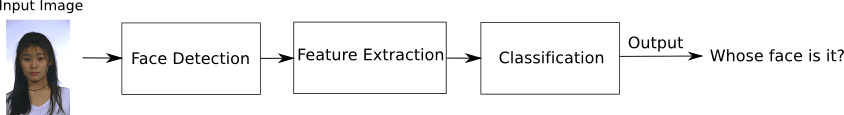
\includegraphics[width=\columnwidth]{ch1/figures/FRS_flowchart.png}
   \caption{The flowchart of three modules of face recognition systems}
    \label{fig:FRSflowchart}
 \end{center}
\end{figure} 
Face detection includes face localisation, segmentation and normalisation, in which a pre-processed face image is obtained from an input scene, either simple or cluttered. Feature extraction derives a representative of the pre-processed face image using a set of features. There are various types of features possibly extracted from the process, such as facial features, statistical appearance-based features, transform coefficient features, algebraic features, etc. In some face recognition systems, there might be a feature selection module between feature extraction and classification. Due to high-dimensionality in the feature space or redundancy among features, such a process is used to select a smaller group of relevant features to represent faces and achieve better recognition performance. Classification is used to assign the above features into one of several categories, \textit{i.e.}, subjects.

Depending on the application context, face recognition can be divided into two scenarios: face verification and face identification. In face verification, an individual who desires to be recognised claims an identity, usually through a personal identification number, an user name, or a smart card. The system conducts a one-to-one comparison to determine whether the claim is true or not, \textit{i.e.}, face verification is to ask a question - ``Does the face belong to a specific person?''. In face identification, the system conducts a one-to-many comparison to establish an individual's identity without the subject to claim an identity, \textit{i.e.}, face identification is to answer the question - ``Whose face is this?''. Throughout this thesis, the generic term \textit{recognition} is used, which does not make a distinction between verification and identification.

\section{Gabor-Boosting algorithm}
Recently, a breakthrough in face detection has been made by Viola and Jones \cite{Viola2001}. Faces are quickly and accurately detected by cascade structured classifiers combined with simple Haar features. In the face detection system, the most significant contribution is the AdaBoost algorithm which selects $200$ most important features from over $180000$ features, and a complex classifier in a cascade structure is built on these important features. The face detector is the most rapid and accurate approach compared to other systems, and it pushes research and development of face detection into a new era. Now many real-time face detection applications, such as those used in digital camera, web cam and mobile phone camera adopt Viola and Jones AdaBoost approach. Facing the big success in face detection, two questions are spontaneously released - ``Can the AdaBoost approach be transplanted into face recognition?'' and if so ``How can the AdaBoost be used in face recognition?''. 
%It leaves the difficulties of face recognition in feature extraction and classification. In the thesis, a face recognition algorithm named \textit{Gabor-Boosting} algorithm is proposed, developed and tested. Gabor wavelet transform is used to extract Gabor wavelet features from face images, Due to very large number of features extracted, AdaBoost is used to select small group of features representing individual's face. After training a classifier with existing faces and their identities, the recognition is done by outputting identities of unknown faces from the classifier. 

This thesis gives an exploration into these two questions. The transplantation of the AdaBoost from face detection into face recognition introduces further sub-questions in feature extraction, feature selection, and classification. These sub-questions are
\begin{itemize}
	\item In face detection, there are only two classes, \textit{i.e.}, face and non-face, so Viola and Jones' work in face detection \cite{Viola2001} is processed using two-class (binary) classification ideas. While, in face recognition, it is more likely there are more than two persons to be discriminated, so that face recognition deals with multiple classes. This prevents the direct transplantation from a two-class environment into a multi-class environment. The solution is to shift face recognition into two-class environments. Hence the sub-question is - ``how can the two-class scenario be established in face recognition?''.
	\item Viola and Jones' approach uses Haar features which are simple so that they can be quickly evaluated. Haar features are sufficient to discriminate differences between face and non-face. However, in face recognition, features are used to discriminate differences between individuals. Obviously, the appearance difference between face and non-face is much larger than the appearance between individuals. Hence, the sub-question is that ``are the Haar features sufficient for face recognition?''. If not, ``what should the substitution be?''.
	\item Within AdaBoost, weak learners (base classifiers)\footnote{Weak learners are the elemental components in AdaBoost training.} are used to evaluate each feature, such that the type of weak learner is a very important factor which determines the performance of AdaBoost. Among the various types of weak learners, ``which types of weak learners are beneficial to improve the performance of face recognition?''.
	\item After the AdaBoost training, a complex classifier is built on weak learners with respect to selected features. The sub-question is: ``is this classifier appropriate for face recognition?''. If not, ``what is the alternative which can be used for recognising human faces?''.
	\item Beside the two-class AdaBoost, there are some multi-class variants of AdaBoost. ``How do these variants fulfil the purpose of multi-class classification from face recognition?''
	\item The AdaBoost approach is very time-consuming \cite{Young2005}. Since images used for face recognition is larger than those images used for face detection in AdaBoost training, the AdaBoost training in face recognition consumes more time than the one in face detection. Hence, there is a sub-question - ``how to reduce the computational time of the AdaBoost training?''.
\end{itemize}

The algorithm described in this thesis is motivated by Viola and Jones' work in face detection \cite{Viola2001}. The algorithm is named \textit{Gabor-Boosting} algorithm, which is proposed, developed and tested. Gabor wavelet transform is used to extract Gabor wavelet features from face images. Due to very large number of features extracted, AdaBoost is used to select a small group of features representing individual's face. After training a classifier with existing faces, the recognition is done by outputting classification results. To evaluate the performance of the Gabor-Boosting face recognition algorithm, the XM2VTS \cite{Matas2000,Messer1999} and FERET \cite{Phillips1997} face databases are used.


%However, there are some differences between face detection and face recognition, which makes applying AdaBoost algorithm difficult on face recognition. In face detection, there are only two subjects, \textit{i.e.}, face and non-face, so Viola and Jones' work in face detection \cite{Viola2001} is processed in a mean of two-class (binary) classification. While, in face recognition, there are many people needed to be recognised, so that face recognition deals with more subjects. The first difficulty is to convert an multiple subjects issue into two subjects issues. In addition, in AdaBoost, weak learners (base classifiers) are used to evaluate each features, such that the type of weak learners is a very important issue which determines the performance of AdaBoost. Different types of weak learners are explored in this thesis, and the optimal type of weak learners is found. In addition, the Gabor-Boosting face recognition is extended from binary classification to multi-class classification with extensions on weak learners and training algorithm. Due to the time-consuming process of AdaBoost, grid computing technology is applied on Gabor-Boosting face recognition, such that the computational time is dramatically reduced. And to evaluate the performance of the Gabor-Boosting face recognition algorithm, the XM2VTS \cite{Matas2000,Messer1999} and FERET \cite{Phillips1997} face databases are used.
In face recognition systems, it is clear that evaluation and benchmarking of the algorithms is crucial. Previous work \cite{Messer1999,Phillips1997,Phillips1998,Phillips2000,Rizvi1998,Rizvi1998fg,Jain2000,Hancock2000,Gauthier2001} on evaluation provides insights into how the evaluation of algorithms and systems can be performed efficiently.  Although great amount of effort has been devoted to face recognition, there are still remains some challenges to be solved such as illumination, head pose, facial expression, occlusion (glasses, sunglasses, scarf, etc), facial hair (beard, mustache, etc.), and ageing. These difficulties make human face appearance in images having very large variations. Therefore, successful face recognition systems have been deployed only under constrained conditions. In this thesis, the face recognition is also deployed under constrained conditions
\begin{itemize}
 \item Illumination is consistent across images
 \item No head pose, but only front-view;
 \item No facial hair and ageing variation, but allowing adequate occlusion (glasses) and facial expression variation.
\end{itemize}
In additional, all images are converted into grey scale.

\section{Thesis Outline}
This thesis is organised as follows: \mbox{Chapter} \ref{ch:review} presents a literature review of face recognition, in which major state-of-the-art techniques of face recognition and face databases are introduced. \mbox{Chapter} \ref{ch:gaboradaboost} gives the background and technical detail of Gabor wavelet transform and AdaBoost. \mbox{Chapter} \ref{ch:FLDAdaBoost} describes the initial Gabor-Boosting face recognition, in which face recognition is converted into two-class classification and Gabor wavelet transform is used to extract human facial features. \mbox{Chapter} \ref{ch:binary} presents a novel weak learner used in AdaBoost training. \mbox{Chapter} \ref{ch:multi} is an extension of the Gabor-Boosting face recognition from a binary domain to a multi-class domain, and also explains how to use grid computing technology to reduce the computational cost of feature selection. The final chapter concludes the work of the Gabor-Boosting algorithm in face recognition, and highlights directions for future work.